The equation of circle can be expressed as
\begin{align}
    \vec{x}^T\vec{x}-2\vec{c}^T\vec{x}+f = 0
\end{align}
$\vec{c}$ is the centre  and substituting the points in the equation of circle we get
\begin{align}
2\myvec{1&2}\vec{c}-f=5\\
2\myvec{2&1}\vec{c}-f=5\\
2\myvec{0&0}\vec{c}-f=0
\end{align}
can be expressed in matrix form
\begin{align}
\myvec{2&4&-1\\4&2&-1\\0&0&-1}\myvec{\vec{c}\\f} = \myvec{5\\5\\0}
\end{align}
Row reducing the augmented matrix
\begin{align}
\myvec{2&4&-1&5\\4&2&-1&5\\0&0&-1&0}
\xleftrightarrow{R_2\leftarrow 2R_1-R_2}
\myvec{2&4&-1&5\\0&6&-1&5\\0&0&-1&0}\\
\xleftrightarrow[R_1\leftarrow R_1-R_3]{R_2\leftarrow R_2-R_3}
\myvec{2&4&0&5\\0&6&0&5\\0&0&-1&0}\\
\xleftrightarrow{R_1\leftarrow 3R_1-2R_2}
\myvec{6&0&0&5\\0&6&0&5\\0&0&-1&0}
\end{align}
\begin{align}
    \vec{c} = \myvec{\frac{5}{6}\\\frac{5}{6}}\\
    f = 0\\
    r=\sqrt{\norm{\vec{c}}^2-f} = \sqrt{\frac{50}{36}}
\end{align}
The required equation of circle is 
\begin{align}
\vec{x}^T\vec{x}-2\myvec{\frac{5}{6}&\frac{5}{6}}\vec{x} = 0
\end{align}
See Fig. \ref{eq:solutions/4/1/2/Fig1}

\begin{figure}[!ht]
\centering
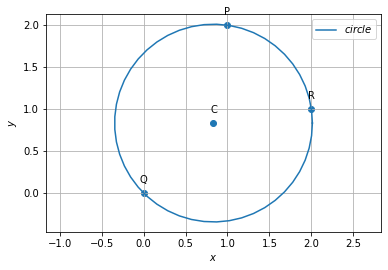
\includegraphics[width=\columnwidth]{./solutions/4/1/2/Circle.png}
\caption{Circle passing through point P,Q,R with centre C.}
\label{eq:solutions/4/1/2/Fig1}
\end{figure}
